\documentclass{article}
\usepackage{graphicx} 
\usepackage{geometry}
\geometry{left=1in, right=1in, top=1in, bottom=1in}
\usepackage{amsfonts}
\usepackage{amsmath}
\usepackage{algorithm}
\usepackage{float}
\usepackage{algpseudocode}
\usepackage{amsmath}
\usepackage{amssymb}
\usepackage{minted}
\usepackage{tikz}
\usetikzlibrary{arrows.meta}
\title{CS 6140 HW2}
\author{Qidian Gao}
\date{Feburary 16th 2024}

\begin{document}

\maketitle

\section{Question 1}
\subsection{a)}
From the lecture we know that this situation happens when 1. The path contains negative value edges, 2. The algorithm doesn't reconsider the distances of previously visited vertices. For example, We can consider the directed graph \(G=(V, E)\), where:
\begin{itemize}
    \item The set of vertices \(V = \{A, B, C\}\)
    \item The set of edges \(E\) consists of:
    \begin{itemize}
        \item An edge from \(A\) to \(B\) with a cost of \(2\) (\(A \rightarrow B = 2\))
        \item An edge from \(B\) to \(C\) with a cost of \(-5\) (\(B \rightarrow C = -5\))
        \item An edge from \(A\) to \(C\) with a cost of \(4\) (\(A \rightarrow C = 4\))
    \end{itemize}
\end{itemize}

Using Dijkstra's algorithm to find the shortest path from \(A\) to \(C\), we initially choose the path \(A \rightarrow C\) directly because it seems to be the shortest with a cost of \(4\). However, the actual shortest path is \(A \rightarrow B \rightarrow C\) with a total cost of \(-3\), which Dijkstra's algorithm fails to identify due to the presence of the negative edge \(B \rightarrow C\).
\begin{center}
    
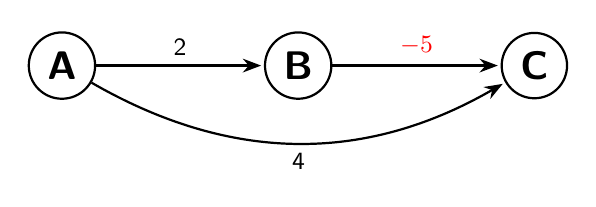
\begin{tikzpicture}[->,>=Stealth,shorten >=1pt,auto,node distance=3cm,
                    thick,main node/.style={circle,draw,font=\sffamily\Large\bfseries}]

  \node[main node] (A) {A};
  \node[main node] (B) [right of=A] {B};
  \node[main node] (C) [right of=B] {C};

  \path[every node/.style={font=\sffamily\small}]
    (A) edge node [above] {2} (B)
        edge [bend right] node [below] {4} (C)
    (B) edge node {${\color{red}-5}$} (C);
\end{tikzpicture}
\end{center}
\subsection{b)}

\subsubsection{Assumption:} Given that $G'$ contains no negative cycles, the shortest path distances $\text{dist}_s(u)$ from $s$ to every node $u$ in $G'$ are well-defined and finite, despite the presence of negative edge costs.\par
\subsubsection{Induction: Triangular Inequality}
For any nodes $u, v \in V$, the principle of the shortest path implies that $\text{dist}_s(v) \leq \text{dist}_s(u) + d(u, v)$. This inequality holds because if there were a cheaper path from $s$ to $v$ through $u$, then it would contradict the definition of $\text{dist}_s(v)$ as the shortest path from $s$ to $v$.


\subsubsection{Proof: }
The reweighting formula for the edge from $u$ to $v$ is $d'(u, v) = d(u, v) + \text{dist}_s(u) - \text{dist}_s(v)$. This adjustment is intended to eliminate negative edge weights, making the graph suitable for algorithms requiring non-negative edge weights.


By the property of shortest paths, rearranging the triangle inequality gives us $d(u, v) \geq \text{dist}_s(v) - \text{dist}_s(u)$. Adding $\text{dist}_s(u)$ to both sides and subtracting $\text{dist}_s(v)$ yields $d(u, v) + \text{dist}_s(u) - \text{dist}_s(v) \geq 0$, which implies that $d'(u, v) \geq 0$.

\subsection{c)}


We consider a graph $G = (V, E)$ with edges that may have negative weights but no negative cycles, and its modified version $G'$ obtained by adding a new node $s$ and zero-cost edges from $s$ to every other node. The cost of an edge $(u, v)$ in $G$ is denoted by $d(u, v)$, and the adjusted cost in $G'$ by $d'(u, v) = d(u, v) + \text{dist}_s(u) - \text{dist}_s(v)$. 

\subsubsection{Proof}


\textbf{Key Argument: }The adjustment of edge costs by $d'(u, v) = d(u, v) + \text{dist}_s(u) - \text{dist}_s(v)$ preserves the relative distances between nodes in terms of shortest paths. This ensures that the optimality of paths remains unchanged between the original and reweighted graphs.

\textbf{If a Path is Shortest in $G$ with $d(u, v)$}

Given a shortest path from any node $u$ to $v$ in $G$, the total cost of this path is minimized using the original weights $d(u, v)$. When adjusted to $d'(u, v)$, the additional terms ($\text{dist}_s(u) - \text{dist}_s(v)$) for each edge on this path effectively cancel out in the sum, except for the start and end of the path, preserving the path's status as shortest.

\textbf{If a Path is Shortest in $G'$ with $d'(u, v)$}

Conversely, if a path minimizes the total adjusted cost using $d'(u, v)$ in $G'$, it also minimizes the original cost using $d(u, v)$ in $G$. The reweighting process does not alter the determination of which path has the smallest cost, as it preserves the relative distances between nodes.
Therefore a path is a shortest path in $G$ using $d(u, v)$ if and only if it is a shortest path in $G'$ using $d'(u, v)$.
\section{Question 2}
\subsection{a)}
\subsubsection{Graph Description}

Consider a simple undirected graph \(G\) with vertices \(A, B, C,\) and \(D\), forming a square with one diagonal. The graph is defined as follows:

\begin{itemize}
    \item Vertices: \(A, B, C, D\)
    \item Edges and their weights: \(AB = 1\), \(BC = 1\), \(CD = 1\), \(DA = 1\), \(AC = 1\)
\end{itemize}

The edges \(AB\), \(BC\), \(CD\), and \(DA\) form the perimeter of the square, and \(AC\) is the diagonal.

\subsubsection{Graph Visualization}
\begin{center}
    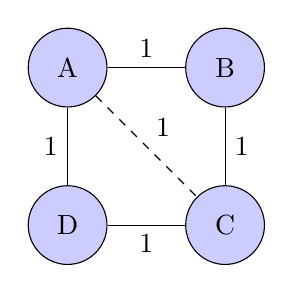
\begin{tikzpicture}[main node/.style={circle,fill=blue!20,draw,minimum size=1cm,inner sep=0pt}, node distance=2cm]
    \node[main node] (A) {A};
    \node[main node] (B) [right of=A] {B};
    \node[main node] (C) [below of=B] {C};
    \node[main node] (D) [below of=A] {D};

    \draw (A) -- node[above] {1} (B);
    \draw (B) -- node[right] {1} (C);
    \draw (C) -- node[below] {1} (D);
    \draw (D) -- node[left] {1} (A);
    \draw[dashed] (A) -- node[above right] {1} (C);
\end{tikzpicture}

\end{center}

\subsubsection{Minimum Spanning Trees}

The graph \(G\) has multiple MSTs, including but not limited to:

\begin{enumerate}
    \item MST 1: Comprising edges \(AB\), \(BC\), \(CD\), and \(DA\), which forms the perimeter of the square.
    \item MST 2: One possible configuration includes edges \(AB\), \(BC\), and \(AC\) plus either of the remaining two perimeter edges not forming a cycle with the chosen edges.
\end{enumerate}

Each MST has a total weight of 3, demonstrating the existence of multiple MSTs for the given graph.

\subsection{b)}
\subsubsection{Assumptions}
Assume that the cost of edges are greater or euqal than 0. Also Assume, for contradiction, that \(T_1\) and \(T_2\) have a different number of edges with the same cost \(c\). Let \(e\) be an edge in \(T_1\) with cost \(c\) not present in \(T_2\).
\subsubsection{Proof}
\begin{enumerate}
    \item Adding \(e\) to \(T_2\) creates a cycle, as \(T_2\) is already a spanning tree. This cycle must contain at least one edge \(f\) not in \(T_1\), since \(T_1\) and \(T_2\) are distinct and \(e\) was not in \(T_2\).
    \item Removing \(f\) from this cycle in \(T_2\) and adding \(e\) yields a new spanning tree \(T_2'\) of \(G\). If the cost of \(f\) is greater than or equal to \(c\), or even if \(f\) has the same cost, replacing \(f\) with \(e\) does not increase the total cost of \(T_2'\), preserving the minimality condition of MSTs.
    \item Repeating this exchange process for any discrepancy in the number of edges with cost \(c\) between \(T_1\) and \(T_2\) would eventually make the two trees identical, contradicting our assumption that they were different.
\end{enumerate}

Therefore, our initial assumption leads to a contradiction, implying that for any cost \(c\), \(T_1\) and \(T_2\) must contain the same number of edges with that cost.
\subsection{c) and d)}
\subsubsection{Assumptions }
Given a graph $G$ with distinct edge weights, we consider an edge $e_0$ in $G$. We aim to design polynomial-time algorithms for:
\begin{enumerate}
    \item[(c)] Deciding whether every minimum spanning tree (MST) of $G$ contains $e_0$.
    \item[(d)] Deciding whether some MST of $G$ contains $e_0$.
\end{enumerate}
It is assumed that the edge costs in $G$ are distinct positive integers, and the running time of our algorithms should be upper-bounded by $O(n^3)$.

\subsubsection{Algorithm for Part (c)}

To decide whether every MST of $G$ contains the edge $e_0$, perform the following steps:
\begin{enumerate}
    \item Remove $e_0$ from $G$ to form the graph $G'$.
    \item Compute the MST of $G'$ using Kruskal's or Prim's algorithm.
    \item If the total weight of the MST of $G'$ is greater than the total weight of the MST of $G$ with $e_0$, then $e_0$ must be in every MST of $G$. Otherwise, it is not.
\end{enumerate}
\begin{algorithm}
\caption{Decide if every MST contains $e_0$}
\begin{algorithmic}[1]
\State $G' \gets G - \{e_0\}$ \Comment{Remove $e_0$ from $G$}
\State Compute MST of $G'$, denote it as $T'$
\State Compute MST of $G$, denote it as $T$
\If {weight($T'$) $>$ weight($T$)}
    \State \Return True \Comment{$e_0$ must be in every MST of $G$}
\Else
    \State \Return False \Comment{$e_0$ is not in every MST of $G$}
\EndIf
\end{algorithmic}
\end{algorithm}
Given the distinctness of edge costs, the MST of $G$ is unique. Removing an edge and finding a new MST with a higher total weight implies the removed edge was part of the unique MST. If the weight does not increase, $e_0$ was not necessary for the MST.

\subsubsection{Algorithm for Part (d)}

To decide whether some MST of $G$ contains $e_0$, simply compute the MST of $G$ using Kruskal's or Prim's algorithm and check if $e_0$ is included.
\begin{algorithm}
\caption{Decide if some MST contains $e_0$}
\begin{algorithmic}[1]
\State Compute MST of $G$, denote it as $T$
\If {$e_0 \in T$}
    \State \Return True \Comment{$e_0$ is in some MST of $G$}
\Else
    \State \Return False \Comment{$e_0$ is not in any MST of $G$}
\EndIf
\end{algorithmic}
\end{algorithm}
With distinct edge weights, the MST is unique. If $e_0$ is included in the MST computed, it indicates that $e_0$ can be part of an MST. Since the MST is unique, this satisfies the condition for "some MST" to include $e_0$.

\section{Question 3}

Given an array of INTEREST scores for $n$ attractions, we aim to find the maximum sum of INTEREST scores from a consecutive subset of attractions. The algorithm should efficiently compute this sum using a divide and conquer approach.

\subsection{Algorithm Description}
The divide and conquer algorithm divides the array into two halves, recursively finds the maximum sum of interest in each half, and then finds the maximum sum that crosses the midpoint, combining these to find the overall maximum.

\subsubsection{Pseudocode}
\begin{verbatim}
Function MaxInterestScore(INTEREST, low, high):
    if low == high:
        return max(0, INTEREST[low])

    mid = (low + high) / 2

    leftMax = MaxInterestScore(INTEREST, low, mid)
    rightMax = MaxInterestScore(INTEREST, mid + 1, high)
    crossMax = MaxCrossingSum(INTEREST, low, mid, high)

    return max(leftMax, rightMax, crossMax)

Function MaxCrossingSum(INTEREST, low, mid, high):
    leftSum = -infinity
    sum = 0
    for i from mid downto low:
        sum = sum + INTEREST[i]
        if sum > leftSum:
            leftSum = sum

    rightSum = -infinity
    sum = 0
    for j from mid + 1 to high:
        sum = sum + INTEREST[j]
        if sum > rightSum:
            rightSum = sum

    return leftSum + rightSum
\end{verbatim}

\subsection{Time Complexity Analysis}
The time complexity of this algorithm is $O(n \log n)$ due to the recursive division of the array into halves and the linear time required to find the maximum crossing sum. Specifically, the recurrence relation is $T(n) = 2T(n/2) + O(n)$, which solves to $O(n \log n)$ by the Master Theorem.

\subsection{Optimization to $O(n)$}
To optimize to $O(n)$, we note that a linear-time Dynamic Programming (DP) approach (Kadane's algorithm) achieves this. However, for the divide and conquer strategy, observing patterns and optimizing the crossing sum computation could potentially reduce unnecessary computations. Yet, achieving $O(n)$ strictly within a classic divide and conquer without additional techniques is challenging.

\end{document}

\end{document}